%%
%% This is file `thesis-ex.tex',
%% generated with the docstrip utility.
%%
%% The original source files were:
%%
%% uiucthesis.dtx  (with options: `example')
%% 
\def\fileversion{v2.25} \def\filedate{2023/01/30}
%% Package and Class "uiucthesis" for use with LaTeX2e.
\documentclass[draftthesis,fullpage]{uiucthesis}
\usepackage{natbib}
\usepackage{hyperref}
\usepackage{graphicx}
\usepackage{etoolbox}
\begin{document}

\title{Small-scale rapid 3D particle tracking}
\author{Liu Hong\\[1cm]{\small Advisor: Leonardo P. Chamorro}}
%\author{Liu Hong}
%\author{Leonardo P. Chamorro}
\department{Mechanical Science and Engineering}
\phdthesis
\advisor{Leonardo P. Chamorro}

\maketitle

\frontmatter

%% Create an abstract that can also be used for the ProQuest abstract.
%% Note that ProQuest truncates their abstracts at 350 words.
%\begin{abstract}
%3D particle tracking is a powerful technique to understand particle %dynamics and complex fluid flow. 
%\end{abstract}

%% Create a dedication in italics with no heading, centered vertically
%% on the page.


%% Create an Acknowledgements page, many departments require you to
%% include funding support in this.
%\chapter*{Acknowledgments}

%This project would not have been possible without the support of
%many people. Many thanks to my adviser, Leonardo P. Chamorro, who
%trained me from a boy lost in research to an independent researcher.
%Without his support and guidance, I can't make so far along the way of %this study. 


%% The thesis format requires the Table of Contents to come
%% before any other major sections, all of these sections after
%% the Table of Contents must be listed therein (i.e., use \chapter,
%% not \chapter*).  Common sections to have between the Table of
%% Contents and the main text are:
%%
%% List of Tables
%% List of Figures
%% List Symbols and/or Abbreviations
%% etc.

\tableofcontents
%\listoftables
%\listoffigures

%% Create a List of Abbreviations. The left column
%% is 1 inch wide and left-justified
%\chapter{List of Abbreviations}

%\begin{symbollist*}
%\item[CA] Caffeine Addict.
%\item[CD] Coffee Drinker.
%\end{symbollist*}

%% Create a List of Symbols. The left column
%% is 0.7 inch wide and centered
\chapter{Introduction}\label{chapter:intro}

Time-resolved3D particle tracking(3D-PTV) is a powerful technique to investigate particle dynamics and complex fluid flows. For particle tracking in common volume($>$10 cm), tomographic approach, which acquires depth information from multiple simultaneous views on illuminated volumes, is a popular method due to its high spatial resolution and
flexibility in the investigation volume. Tomographic approach usually involves four steps, particle reconstruction, track initialization, prediction and optimization. Although previous researchers proposed advanced prediction and optimization method, such as iterative particle reconstruction (IPR) \citep{wieneke2012iterative} and Shake-The-Box \citep{schanz2016shake}, numerous ghost particle created during the triangulation limits its application in industry area. This study first gets inspired by optimizing 4 views triangulation task, which is further described in \hyperref[chapter:DLT]{Patallelized DLT} chapter, focuses on small scale particle tracking.

% * This part I use the paragraph from my Lab on Chip paper
The sustained progress on microfabrication techniques in the last couple of decades has opened new possibilities for microfluidics and, in particular,  the design of biomedical devices and control of processes, including cooling \citep{singhal2004microscale}, mixing  \citep{song2003millisecond,liu2004two}, extraction \citep{hisamoto2001chip, kluge2009production} and drug delivery \citep{tsai2007review, nguyen2013design}. Hence, demands of tracking particle in small volume have increased. In order to overcome illumination and space constraints, techniques based on standard particle tracking, such as holographic \citep{sheng2006digital, soria2008towards, memmolo2011twin, daloglu2018label}, confocal \citep{kinoshita2007three, lima2008vitro}, stereoscopic \citep{lindken2006stereoscopic, bown2006three} and defocus-based \citep{yoon20063d, pereira2007microscale} variants; see discussion in \citet{wereley2010recent}. Development of microlens manufacturing technology and camera sensing allows for distinct possibilities for taking advantage of the so-called light field, LF \citep{gershun1939light}, which describes the distribution of light rays in space instead of 2D projection, in plenoptic function models  \citep{adelson1991plenoptic}.

Light field cameras have been used in  photography \citep{levoy1996light, ng2005fourier}, computer vision \citep{tao2013depth, adelson1992single} and robotic navigation \citep{kaveti2020light}, among others. \citet{belden2010three} used concepts of LF imaging in a large camera array to capture multiple views simultaneously. Unlike tomo-PIV, \citet{belden2010three} performed synthetic aperture refocusing, which was coined as synthetic aperture particle image velocimetry, SA-PIV, by using a map-shift-average algorithm. The large number of cameras needed may make it relatively bulky and costly.    

Instead of considering a multi-camera approach, the use of microlens array, MLA, into the optical train of a conventional microscope  \citep{levoy2006light} has enabled the application span of LF to micro scale with a single, high-resolution camera. LF also has several advantages compared to SA-PIV or tomo-PIV. Indeed, the camera spatial calibration process, which is difficult in microscopic measurements, is unnecessary when MLA is pre-calibrated with a CCD or CMOS sensor. The relative independence of the main optic system leads to the LF technique being widely applied to a variety of microscopes and macro lenses and providing robust 3D data. Single-camera light field micro particle velocimetry, LF-PIV, proposed by Lynch et al. \cite{lynch2012three} became a popular complementary approach for space-constrained measurements \citep{shi2016dense, shi2016parametric, shi2017light, fahringer2015volumetric, xu20173d, li2017investigation}. 
Indeed, there are other single-camera methods, such as digital holography. Unfortunately, comparatively high-power laser requirement \citep{hinsch2002holographic} and low signal-to-noise ratio \citep{ooms2009digital}, and long reconstruction time may limit applications.


Despite this, several bottlenecks limit the capability and development of LF-PIV. One of the main drawbacks is the high computational cost during 3D reconstruction. Like conventional tomo-PIV, the space is discretized into cubic voxels with associated intensity and optic system project $E(x,y,z)$ onto 2D pixel-wise intensity distribution $I(x,y)$ \citep{fahringer2015volumetric}, as follows:
\begin{equation}
  \sum_{j \in N_{i}} w_{i,j} E\left(x_j, y_j, z_j\right)=I\left(x_i, y_i\right),
  \label{LF_principle}
\end{equation}
where $N_i$ indicates the number of voxels in the line-of-sight of the $i-$th pixel, and $w_{i,j}$ represents a weighting coefficient dependent on the optic system. This is an ill-posed problem caused by an under-determined system of equations. A special series of algorithms known as algebraic methods that iteratively solve this linear equation system were introduced by \citet{herman1976iterative}. For example, the standard multiplicative algebraic reconstruction technique, MART, proposed by \citet{belden2010three} is widely utilized with appropriate modifications to calculate the voxel intensity:
\begin{equation}
       E\left(x_j,y_j,z_j\right)^{k+1}=E\left(x_j,y_j,z_j\right)^{k}\left(\frac{I\left(x_i, y_i\right)}{\sum_{j \in N_j} w_{i,j} E\left(x_j, y_j, z_j\right)^k}\right)^{\mu w_{i, j}}.
       \label{LF_MART}
\end{equation}

Here, $k$ is the iteration number, and $\mu$ is a relaxation factor. Many pixels can capture one voxel, leading to an extended processing time in the weight matrix calculation and iterative steps. For instance, saving non-zero values of a 300 $\times$ 200 $\times$ 200 voxels and 850 $\times$ 850 pixels weighting matrix requires approximately 350 GB, which is substantial for standard computers. 3D reconstruction for low-resolution image examples may still take on the order of an hour on a 12-core workstation with RAID 0 solid-state disk array.  Other methods, including the so-called dense ray tracing-based MART \citep{shi2017light} and pre-recognition simultaneous algebraic reconstruction technique \citep{zhu2021pre}, have been proposed to improve the efficiency of reconstruction. However, the assessment of the weighting matrix bottleneck remains significant.  


Consider sparse particle concentration characteristic for small-scale particle tracking and orthographic view of microscope, \citet{levoy2006light} and \citet{ truscott2017three} utilized a 3D deconvolution algorithm to remove blurring effects in the images focal stack. 
Compared to algebraic methods, 3D deconvolution is efficient since it avoids storing large weighting matrices. However, iterative deconvolution such as the Richardson-Lucy algorithm \citep{sibarita2005deconvolution} uses substantial computational power to store a focal stack of images and perform voxel-wise deconvolution. Like the kernel of deconvolution, point-spread-function (PSF) estimation needs the absence of noise and aberrations by empirically refocusing a sub-resolution fluorescent particle at the center of a lenslet \citep{levoy2006light}. It may not be convenient to image sub-resolution fluorescent particle with the same optical system as a PIV setup, leading to inappropriate PSF estimation. PSF is not invariant to translation, making it inappropriate to use one PSF to deconvolve all voxels \citep{zhu2021pre}. Regardless of the performance of the algorithm, alignment between pixels of sub-images and MLA, which ensure a consistent square matrix of pixels underneath each lenslet and MLA rotated to axis-align with the camera sensor, is difficult to achieve during calibration due to lens distortion and fall of intensity towards the periphery of an image \citep{piller2012microscope}.

% * Finish citing from Lab on Chip paper

Here, this study extends the application of non-terative ray tracing 3D microscale particle tracking ( \hyperref[chapter:MPT]{Microscale Particle Tracking}) to cm-scale (\hyperref[chapter:cm]{Cm-scale 3D Particle Tracking})since fluid field and particle motion and particle motion are more complex and harder to simulate compare to microscale. \hyperref[chapter:cm-scale]{Cm-scale 3D Particle Tracking} 
describes the major challenges faced for using this approach with perspective view system.  

\renewcommand{\cleardoublepage}{} %TODO remove those two lines if not reach 20 page
\renewcommand{\clearpage}{}
\chapter{Parallelized DLT - Inspire}\label{chapter:DLT}
In this work, 4 calibrated camera system was employed to acquire 3D trajectories of grains inside the harvester to optimize the shelling and separating process. Charuco board \citep{an2018charuco} based intrinsic and extrinsic calibration method was used to simplify calibration procedure and improve the robustness. Parallelized direct linear transformation (DLT) was utilized to remove the ghost particles and compute the 3D position of particle candidates. This algebraic 4 ray intersection method inspires later works of $N$ rays intersection approach. 
\subsection*{Experiment Setup and Principal Of 3D Tracking}
4 a2A1920-160umBAS camera were mounted to capture image sequences for investigation volume from various view points. The camera system was calibrated by capturing 1000 frames of 7 $\times$ 10, grid size 20 mm charuco board whose position was altered in the meanwhile. First, each camera intrinsic parameter $K$ and distortion coefficients $d$ were calibrated from corresponding image sequence.
Using 2D-2D correspondences about unique charuco board corners, relative pose of each camera pair $X_j = R_{ij}X_i + T_{ij}$, where $R_{ij}$ is rotation matrix and $T_{ij}$ is translation vector, in 4 camera can estimated. By fixing the first camera coordinate system as real world coordinate system, $R_1 = I_{3 \times 3}$, $T_1 = (0,0,0)^T$, poses of 4 camera were registered into real world coordinate system. A camera graph $G$ with minimum degree $\delta (G) \geq 2$ is formed and tuned by bundle adjustment \citep{engels2006bundle}.   
Once the 4 camera system got calibrated, the beans were released above the investigation volume and synchronized image sequences were captured with 150 fps.

Figure \ref{fig:DLT} describes the calibrated 4 camera system. A beam with real world coordinate $(x,y,z)$ was captured by 4 cameras with corresponding image coordinates $(u_1,v1)$, $(u_2,v_2)$, etc. Referring to pinhole camera model, the relationship between particle image coordinates and real world coordinates in homogeneous coordinate system is governed by 

\begin{equation}
       \left[\begin{array}{c}
              u_i \\
              v _i\\
              1
              \end{array}\right]=K_i\left[\begin{array}{ll}
              R_i & T_i
              \end{array}\right]\left[\begin{array}{c}
              x \\
              y \\
              z \\
              1
              \end{array}\right] = \left[\begin{array}{c}
                     \overrightarrow{P_{i,1}}\\
                     \overrightarrow{P_{i,2}}\\
                     \overrightarrow{P_{i,3}}
              \end{array}\right] \left[\begin{array}{c}
                     x \\
                     y \\
                     z \\
                     1
                     \end{array}\right]      , i = 1,2,3,4,
\end{equation}
where $\overrightarrow{P_{i,i=j}}$ is $j^{th}$ row vector of projection matrix \textbf{$P_i$}. Based on DLT algorithm \citep{shapiro1978direct}, real word particle position vector $\overrightarrow{X}$ can be solved by minimizing $\vec{w}$ :
\begin{equation}
       A \vec{X}=\left[\begin{array}{c}
       v_1 \vec{p}_{1,3}-\vec{p}_{1,2} \\
       \vec{p}_{1,1}-u_1 \vec{p}_{1,3} \\
       v_2 \vec{p}_{2,3}-\vec{p}_{2,2} \\
       \vec{p}_{2,1}-u_2 \vec{p}_{2,3} \\
       \vdots
       \end{array}\right] = \vec{w} \approx 0,
\end{equation}
where $\vec{w}$ is residue induced by noise. With SVD decomposition of $A$,  $\overrightarrow{X}$ will be the corresponding column vector of $V^T$ with smallest value of $s$. 
\begin{figure}[h]
       \centerline{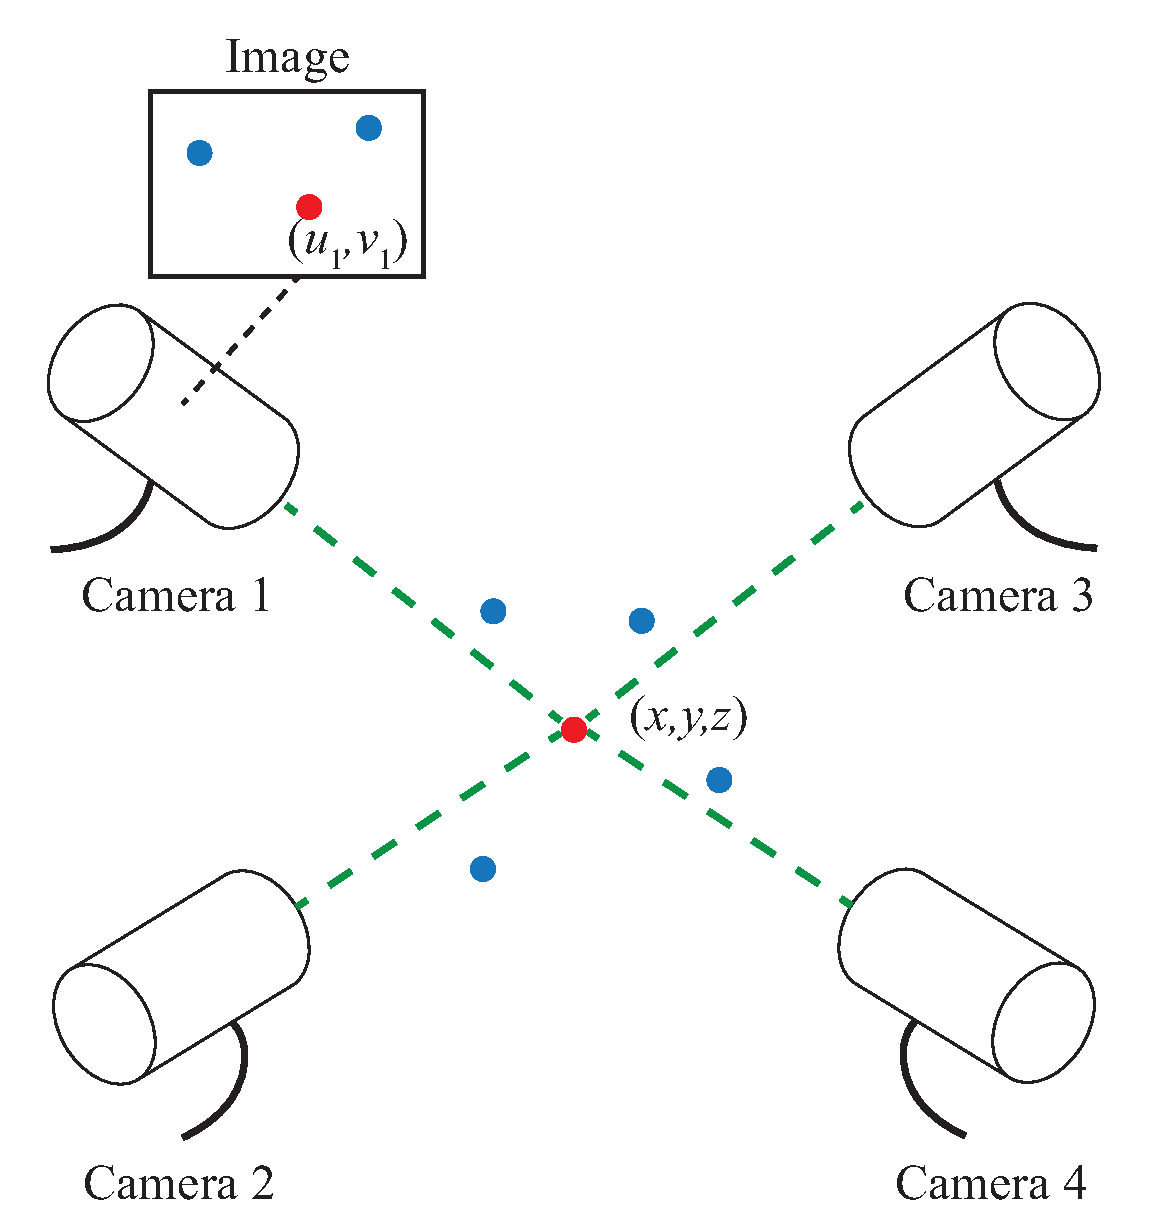
\includegraphics[width=0.6\linewidth]{FIG/DLT.eps}}
       \caption{4 view 3D particle reconstruction.}
       \label{fig:DLT}
\end{figure}
Due to weak matching between views for 2D particle detection, $\overrightarrow{X}$ candidates and corresponding $s$ were computed by DLT method with OpenMP optimized SIMD instruction. Ghost particle positions were removed according to descending order of $s$. Linking algorithm, proposed by \citet{crocker1996methods}, was utilized to further remove outliers.

\subsection*{Result and Remark}
This work achieved 4 view 3D particle tracking in large domain nearly instantaneously by removing majority of ghost particle during triangulation process. The basic principle about reconstruct particle based in $N$ ($N = 4$) rays inspired following small scale particle tracking study.


\chapter{Microscale Particle Tracking - Prototype}\label{chapter:MPT}
This Chapter is from the Journal Article:
Hong, Liu, and Leonardo P. Chamorro. "A fast, non-iterative ray-intersection approach for three-dimensional microscale particle tracking." \textbf{Lab on a Chip} 22.5 (2022): 964-971.

In this work, we propose a non-iterative ray tracing method with robust post-capture microlens array sensor alignment to reconstruct sparse particle concentration in light field particle image velocimetry and particle tracking velocimetry nearly instantaneously. Voxels traversed by various rays are stored by kd-tree to reduce memory load and computational time. Cloud point classification algorithm is employed for particle identification and spatial reconstruction. The approach is tested with a physically-based realistic model of a light field camera. Also, an optical system is assembled in a microscope to directly obtain the 3D laminar velocity field in the fully-developed region, which exhibits good agreement with the theoretical solution.

\subsection*{Light Field Microscopy}
Consider placing a microlens array in the intermediate image plane between a tube lens of an infinity-corrected microscope and a camera sensor to enable the microscope capturing light field in a single photograph \citep{levoy2006light}; see a basic diagram in figure \ref{fig:lf_principle}.

\begin{figure}[h]
       \centerline{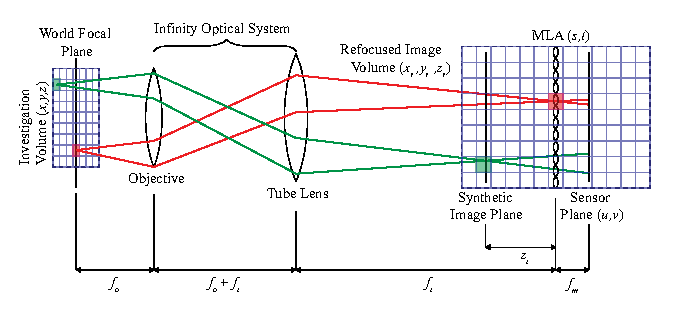
\includegraphics[width=1\linewidth]{fig/LFM.eps}}
         \caption{Schematics of a Light field system with an infinity-corrected microscope. Red lines indicate rays from in focus particle, whereas green lines denote those for an out-of-focus particle.}
       \label{fig:lf_principle}
\end{figure}

A 4D array $L(u,v,s,t) $ \citep{levoy1996light} describing the intersection of rays between sensor ($u,v$) and MLA ($s,t$) planes can be converted from a raw light field image.  The sensor plane is located at the focal plane of MLA with a distance equal to the focal length of the lenslet $f_l$. The $(u,v)$ coordinates are associated with pixels in each lenslet, encoding angular information. The $(s,t)$ coordinates are associated with the center of each lenslet and encode spatial information. In each sub-image in $(u,v)$ coordinates, the lenslet center is identified as origin (0,0).

Due to it is not practical to perfectly align the lenslet center with a pixel in the camera sensor, pixels in each lenslet are interpolated onto a uniform $(u,v)$ grid for computational efficiency. By decoding the 4D array $L(u,v,s,t)$, depth information can be recovered at the expense of spatial resolution \citep{levoy2006light}. For this 3D reconstruction approach, the spatial resolution is modulated by the size of lenslet $d_m$, whereas the depth resolution is governed by the sub-image resolution $N_s = d_m / d_p$, where $d_p$ is the pixel size.  Once 2D raw light field images are reshaped to a 4D array, 3D intensity distribution can be calculated using algebraic or 3D convolution methods. 

Since the majority of pixels do not receive rays from the particles and PIV/PTV only need to reconstruct the location of the particles, rays unit vector pre-filtered data matrix $Q$ (\autoref{unit_vector}) and rays counter matrix $C(x_r,y_r,z_r)$ are introduced to reduce the computational load. A simple intensity threshold filter computed based on raw images without particles 
may be used to binarize light field images to select pixels lit by particles to form
\begin{equation}
       Q=\left[\begin{array}{ccccc}
       \mid & \mid & \mid & \mid & \mid \\
       x_p & y_p & \hat{i} & \hat{j} & \hat{k} \\
       \mid & \mid & \mid & \mid & \mid
       \end{array}\right], \quad Q \in C^{M \times 5}
       \label{unit_vector}
\end{equation}
where $M$ indicates the number of rays used for ray tracing, $(x_p, y_p)$ is the pixel coordinates on the sensor and $(\hat{i}, \hat{j}, \hat{k})$ is the unit direction vector given by connecting the pixel and its corresponding lenslet center treated as a pinhole.

Then, the 3D reconstruction of particles can be converted to an "intersection points" finding problem (figure \ref{fig:ray_counter}a) of 3D skew lines (Rays). The refocused image volume is discretized into small voxels, and the ray counter matrix $C(x_r,y_r,z_r)$ is zero-initialized to solve this problem. Since all rays are nearly perpendicular to the ($x,y$) plane, we consider that a ray can be conceptualized as passing through the voxel if it intersects with the center plane of the voxel (figure \ref{fig:ray_counter}b) to accelerate calculation. The spatial coordinates of intersected points for rays with different depth center planes can be computed as follows:
\begin{equation}
  \left[\begin{array}{c}
    {x_p}^{\prime} \\
    {y_p}^{\prime}
    \end{array}\right]=\frac{z_r}{\hat{k}}\left[\begin{array}{c}
    \hat{i} \\
    \hat{j}
    \end{array}\right] + 
    \left[\begin{array}{c}
    x_p \\
    y_p
    \end{array}\right]
  \label{eq:intersection}
\end{equation}

Using a binary search, the rays counter of the closest voxel $(x_r,y_r,z_r)$ of the intersection point $(x_p’, y_p’, z_r)$ is incremented by one. The counting is performed with atomic operation in GPU's shared memory to reduce processing time  (figure \ref{fig:ray_counter}b). The ray counter matrix $C(x_r,y_r,z_r)$ is filtered by half of the number of pixels lit by a particle in-focus plane to avoid noncritical cloud point processing; it is computed as
\begin{equation}
    C_{min} =  \lfloor \frac{1}{2}(R_p \times M / q)^2 \pi \rfloor,
  \label{eq:RayCounterThreshold}
\end{equation}
where $\lfloor x \rfloor$ is the floor function,  $M$ is the magnification of the objective lens, $R_p$ is the radius of the particle, and $q$ is the pixel size. Then, according to the particle density in the discretized refocused image volume, sparse voxels with ray counters can be classified and further reduced to a one-to-one correspondence between particles and voxels. If points cloud are relative dense, voxels with local maximum ray counters are screened with a fast nearest neighbor search of kd tree \citep{ramasubramanian1989generalized}. Otherwise, density-based spatial clustering of application with noise, DBSCAN \citep{ester1996density} is utilized to classify voxels, and the center positions are computed via averaging throughout classes. See the illustrative flowchart in figure \ref{fig:flowchart}.

\begin{figure}[h]
       \centerline{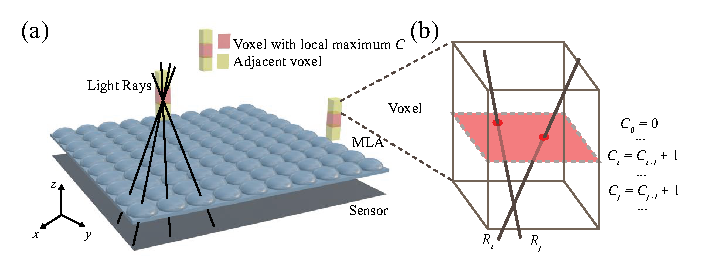
\includegraphics[width=0.7\linewidth]{fig/figure2.eps}} 
       \caption{(a) 3D light ray diagram of an image volume around the microlens array, MLA; (b) increment of ray counter in one voxel.}
       \label{fig:ray_counter}
\end{figure}
       
       
\begin{figure}[h]
       \centerline{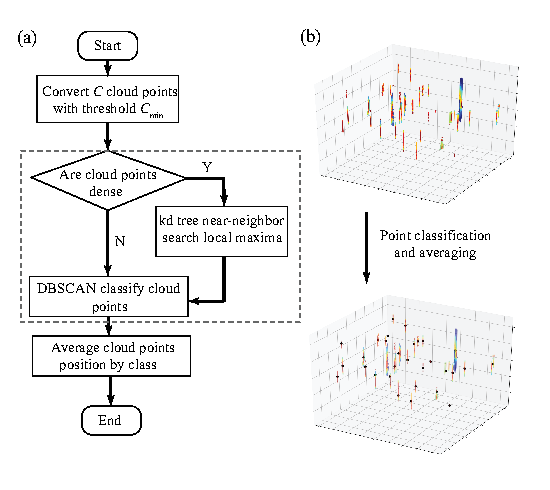
\includegraphics[width=0.7\linewidth]{fig/figure3.eps}}
       \caption{(a) Cloud point classification and center position calculation flowchart; (b) 3D cloud point for particle center position calculation.}
       \label{fig:flowchart}
\end{figure}

\section*{Ray simulation}\label{sec:simulation}
Now, we introduce a physically-based simulation \citep{michels2018simulation} with a realistic lens to compare the ground truth with a refocused position of particles. An $f/2.0\pm 22^{\circ}$ double-Gaussian camera lens is constructed in Blender, as shown in figure \ref{fig:simulate_lens}a. All the surfaces of the objective lens are discretized into 64 radial and 128 longitudinal vertices to achieve an approximately round surface, and a material shader is used for normal surface correction. Details of this particular lens can be found in \citet{smith2005modern}. With 2D Ray simulation in Zemax, the optic system can be treated as a thick convex lens with two cardinal planes $H_1$, $H_2$ as illustrated in figure \ref{fig:simulate_lens}b. 
\begin{figure*}[h]
       \centerline{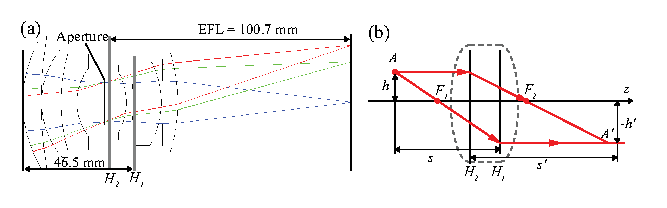
\includegraphics[width = 0.8\linewidth]{fig/figure4.eps}} 
        \caption{(a) Schematics of the double-Gaussian camera model with MLA;  (b) an equivalent thick convex lens with two cardinal planes, $H_1$ and $H_2$.}
      \label{fig:simulate_lens}
\end{figure*}
\begin{figure*}[h]
       \centerline{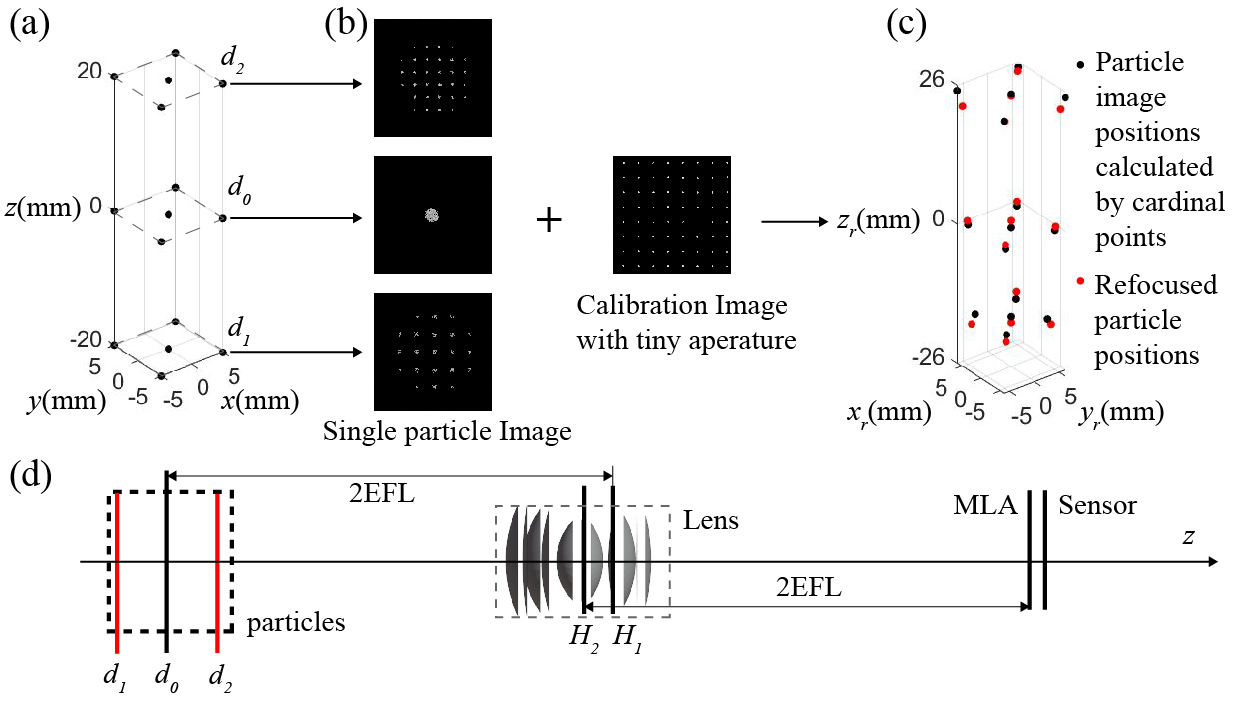
\includegraphics[width=0.8\linewidth]{fig/figure5.jpg}}
       \caption{Configuration of LF simulation for uncertainty analysis of 3D particle reconstruction. (a) Three layers of particles in the objective space; (b) corresponding LF images; (c) reconstruction with ground truth; (d) Simulation details.}
       \label{fig:simu}
\end{figure*}
The scattered light from an object in position $A$ has a corresponding image position $A^{\prime}$ calculated as follows:
\begin{equation}
  \frac{1}{EFL} = \frac{1}{s^{\prime}} + \frac{1}{s}
\label{eq:z_image}
\end{equation}
\begin{equation}
  \left[\begin{array}{c}
    {x_i} \\
    {y_i}
    \end{array}\right]=\frac{s^{\prime}}{s}\left[\begin{array}{c}
    x \\
    y
    \end{array}\right] 
  \label{eq:xy_image}
\end{equation}
where EFL is the effective focal length. All other parameters used in this simulation are based on the experiment's device to compare with a real experimental setup. A rectangular MLA with pitch $p_m$ = 125 $\mu$m and focal length $f_m$ = 3.75 mm is placed at 2$EFL$ behind the $H_2$ plane. The curvature radius $R_1$ of each lenslet of the MLA with negligible thickness of backplate, $d \approx 0$, and flat backplane, $R_2 = \infty$, is computed based on the lens maker's equation
\begin{equation}
  \frac{1}{f_m}=(n-1)\left(\frac{1}{R_{1}}-\frac{1}{R_{2}}+\frac{(n-1) d}{n R_{1} R_{2}}\right)=\frac{n-1}{R_{1}}.
\label{eq:lensmaker}
\end{equation}
Here, $n = 1.56$ is the index of refraction, IOR, according to the MLA material (MLA-S125-f30) used in the experiment. A $35.9$ mm $\times$ $23.9$ mm camera sensor with 8256 pixels $\times$ 5504 pixels (Nikon D850), is placed on the focal plane of the MLA as shown in figure \ref{fig:simu}d.

Spherical particles of radius $r=30$ $\mu$m are placed at various depths $z$, namely, $d_0$, $d_1$,  and $d_2$ in figure \ref{fig:simu}d) with a distance of around 2$EFL$ from the $H_1$ plane. Based on equation \ref{eq:z_image}, the in-focused particles image is located in the MLA plane. Emission shade is added to the particle's surface to simulate light reflection or emission in a real experiment. By using implemented cycles render engine, 2048 render samples per pixel are computed with GPU. Three raw LF images are rendered corresponding to 15 particles on the $d_0$, $d_1$ and $d_2$ planes. Figure \ref{fig:simu}a shows the particle positions in the objective volume, and figure \ref{fig:simu}b shows the raw counterpart. Then, a calibration image is rendered by creating an area light source on $d_0$ and reducing the aperture size of the main lens to a sufficiently small value. 

The image volume is discretized into 125 $ \mu$m ($x$) $\times$ 125 $\mu$m ($y$) $\times$ 250 $\mu$m ($z$) voxels and the corresponding ray counter matrix $C(x_r,y_r,z_r)$ is initialized. Finally, the 3D particle positions are reconstructed to voxels in the image volume and compared with theoretical image positions calculated from equation \ref{eq:z_image} and \ref{eq:xy_image}; see figure \ref{fig:simu}c. The mean error distance in image volume is 1.24 mm; it is caused by lateral resolution, limited angular resolution, radial distortion, depth distortion, vignetting, and the limited number of simulated rays. However, high magnification and tele-centricity (orthographic views) of the macro lens and microscopes can reduce distortion induced by the lens. All rays that go through MLA are recorded by pixels in the real experiment. The distance error in object volume should be recomputed based on the lens magnification, $M$, i.e., 
\begin{equation}
  \Delta x = \frac{\Delta x_i}{M}, \Delta y = \frac{\Delta y_i}{M}, \Delta z = \frac{\Delta z_i}{M^2}
\label{eq:error}
\end{equation}
where $\Delta x_i$, $\Delta y_i$, and $\Delta z_i$ are distance errors in the image volume, whereas $\Delta x$, $\Delta y$, and $\Delta z$ are distance errors in the object volume. For instance, with a 20X objective lens, 1.24 mm distance error under a large lens distortion leads to an only upper bound of 10.6 $\mu$m distance error (around 10$R_p$) in the objective volume. The distance error of particle 3D reconstruction of the microscope is much smaller compared to the simulation case.

\section*{Experiment - Proof of concept}
3D PIV is conducted in a rectangular micro channel of 200 $\mu$m $\times$ 200 $\mu$m cross-section and $\times$ 58.5 mm long; see basic schematics  in figure \ref{fig:setup}a. The system uses a Nikon Eclipse Ti2 inverted microscope, which utilizes fluorescence filter cubes to capture high signal-to-noise ratio images. A Nikon CFI Plan Fluor 20X/0.5 objective lens is used to provide high contrast fluorescence observation, and a 45.4 megapixel Nikon D850 camera (pixel size $p=4.35$ $\mu$m) with nose-to-nose 50 mm f/1.8D lenses is employed to capture 1:1 images with large aperture. A 25.4 mm round MLA (RPC photonics S125-f30) contains lenslets with pitch size $p_l$ = 125 $\mu$m and focal length $f_m$ = 3.75 mm. 
A continuous 532 nm laser is used to illuminate the interrogation volume through a dichroic filter cube and objective lens. The seeding consists of 1.7-2.2 $\mu$m fluorescent Nile Red particles (Spherotech), whose emission spectral peak is around 560 nm. A high-pass filter in the cube blocks the reflections of the laser light and allows emission light from particles capture from the camera. A programmable Harvard syringe pump pumps a distilled water-particle solution to the microchannel through microtubes at a flow rate of  0.85 $\mu$l/min (equivalent to a Reynolds number of $Re\approx 0.07$). Thirty-five images are captured at a low frame rate of 7 Hz with DX-format, 300 $\mu$s exposure and 25600 ISO to maximize image resolution without binning.  See a diagram and photograph of the setup in figure \ref{fig:setup}.

This configuration implies a minimum number of spots behind each lenslet $N_u\approx$ 23.7 \citep{levoy2006light}, which is calculated as,
\begin{equation}
  N_u = \frac{p_l}{R_{obj}}, R_{obj} = \frac{0.47\lambda}{NA}M
\label{eq:Nu}
\end{equation}
where $\lambda$ is the emission wavelength of fluorescent particles, $NA$ is numerical aperture, $M$ is magnification of objective lens and $R_{obj}$ is the Sparrow limit for the smallest spacing between two distinguishable spots in the specimen \citep{inoue2013video}. The number of pixels in one lenslet,  $p_l/p\approx 28.7$, is larger than $N_u$ to ensure the pixel density does not limit the angular resolution. $N_u$ can also be regarded as the number of slices in the depth direction, leading to a depth resolution $D_{tot_2}$ $\approx$ 28.8 $\mu$m and a total reconstruction depth $D_V\approx 680$ $\mu$m \citep{levoy2006light}, which are computed as,
\begin{equation}
  D_{tot_2} \approx \frac{(2 + N_u)\lambda n_m}{2NA^2}, D_V \approx N_uD_{tot_2}
\label{eq:DtotAndDV}
\end{equation}
where $n_m$ is refractive index of the medium. 
To simplify the problem and to avoid under-sampling, the depth length of voxel for image volume is set to $\Delta z_r$ $\approx$ $D_{tot_2}M^2/3$ $\approx$ 4 mm. Furthermore, $\Delta z_r$ ($\approx 4$ mm) also prevents reconstruction from virtual image since it is larger than $f_m$. 
\begin{figure}[h]
       \centerline{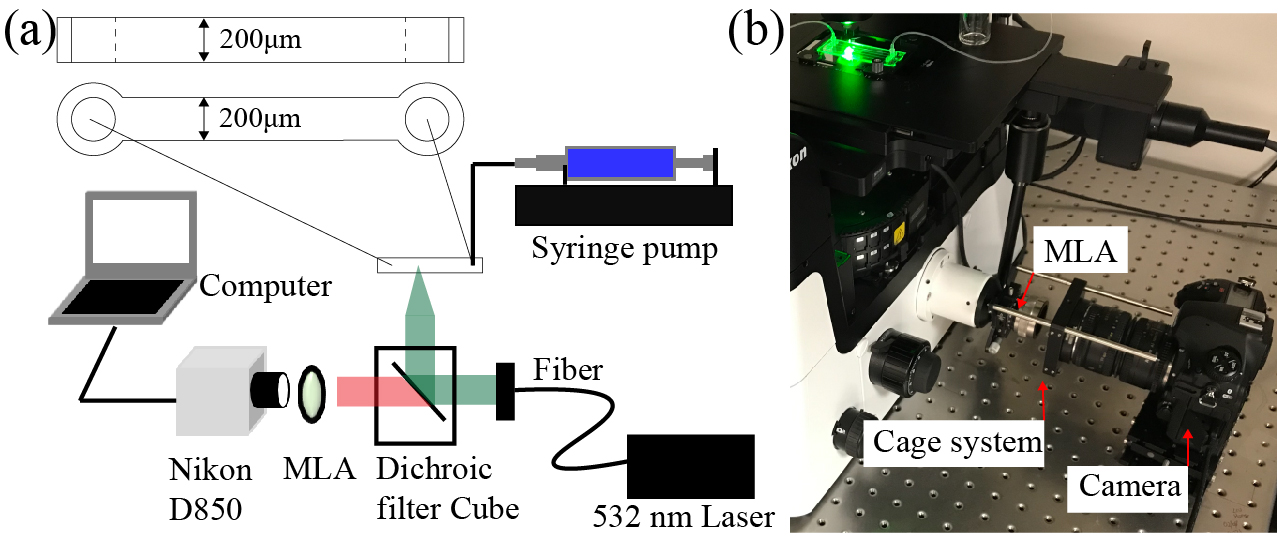
\includegraphics[width=0.8\linewidth]{fig/figure6.jpg}}
       \caption{(a) General schematic of the microchannel and experimental setup; (b) photograph of the pre-calibrated MLA cage system by placing the MLA into intermediate image plane between 1:1 DSLR camera and microscope.}
       \label{fig:setup}
\end{figure}

\section*{Result and Discussion}
The  LF 3D$-\mu$PIV is compared with the theoretical fully-developed laminar solution for the flow rate of 0.85 $\mu$l/min.
Figure \ref{fig:result}a illustrates velocity profile colored with velocity magnitude. A comparison of the velocity profiles along the major diagonals are shown in figure \ref{fig:result}b,c. The maximum velocity magnitude from the experiment match well with the theoretical prediction. However, some departures are attributed to image plane too close to the MLA plane. Shorter $f_m$ offers more accurate reconstruction around the MLA plane, but it sacrifices depth of view. Furthermore, high particle velocity in center region also destabilizes the linking algorithm, which may also affect estimation of the velocity field. Finally, the relative measurement error is calculated as
\begin{equation}
  e(y,z) =  \frac{\left| u_{exp}(y,z) - u_{theo}(y,z) \right|}{u_{theo}(y,z)} \times 100
\label{eq:Uncertainty}
\end{equation}
where $u_{exp}(y,z)$, $u_{theo}(y,z)$ are velocity profile based on experiment and theoretical prediction.
As a result, the relative error is around 5$\%$ in the corner region and 12 $\%$ at the center. Overall, the bulk flowrate is estimated as 0.834 $\mu$m/min, close to the experimental flowrate of 0.85$\mu$m/min.
\begin{figure}[h]
       \centerline{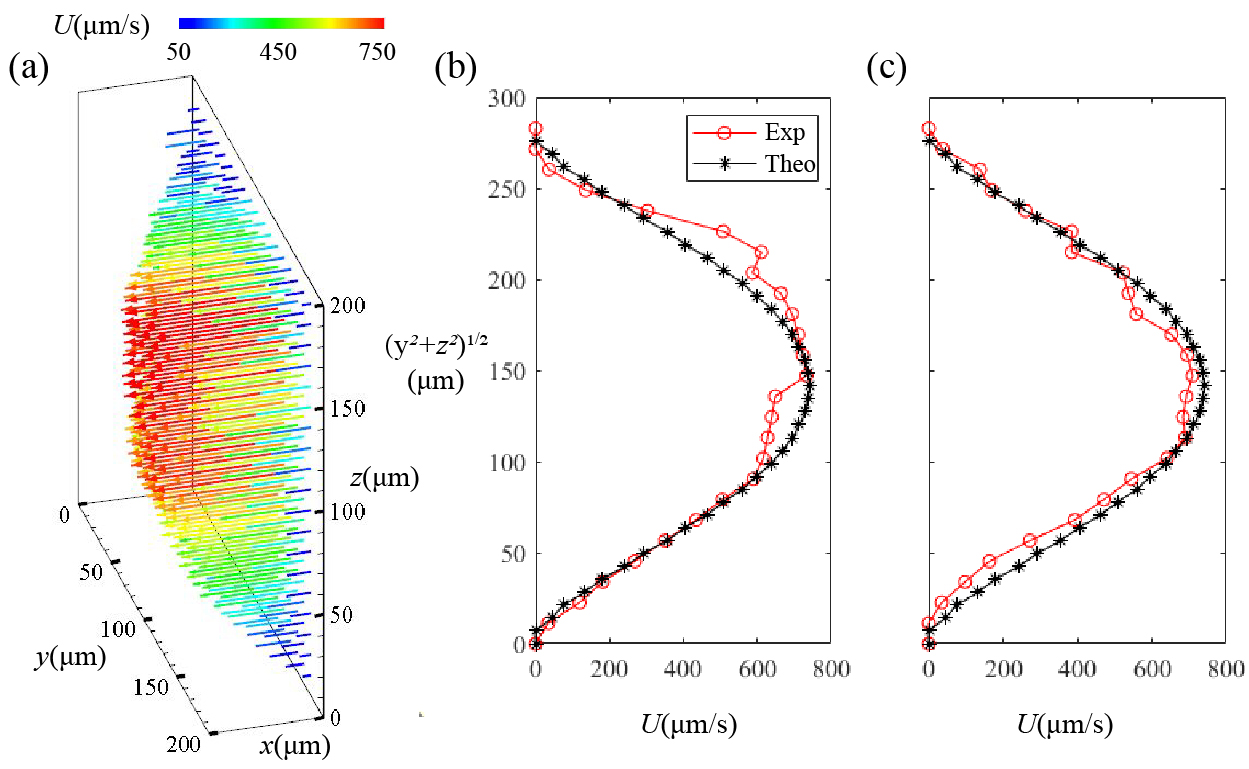
\includegraphics[width = 0.7\linewidth]{fig/figure8.jpg}} 
       \caption{(a) A view of the velocity distribution; (b) comparison of the measured velocity profile along the $y-z$ diagonal direction with theoretical profile; (c) same as b) but in the other diagonal.}
     \label{fig:result}
\end{figure}

\chapter{Cm-scale 3D Particle Tracking - Propose}\label{chapter:cm}
Multi-camera-based flow description in Eulerian and Lagrangian frames of reference at mm and cm scales is usually challenging due to shallow depth of field (DOF) from macro lenses and calibration procedures. I want to improve the rapid 3D particle tracking system described in above chapter for cm-scale volume application with perspective view. With the use of a microlens array (MLA) in the intermediate plane between the macro lens and camera sensor (\autoref{fig:ZoomLens_Setup}), light field information can be obtained by a single camera cage system without stereo calibration. A fast ray intersection and cloud point classification method with GPU acceleration is applied to reconstruct 3D particle position in a uniformly discretized image space and then mapped to non-uniform objective space based on macro lens properties. With atomic operation within the onboard memory of GPU, the processing time per image can be under one second. Lagrangian particle tracking Crocker-Grier method is used for particle linking to characterize time-resolved flow field.

\begin{figure}[h]
  \centerline{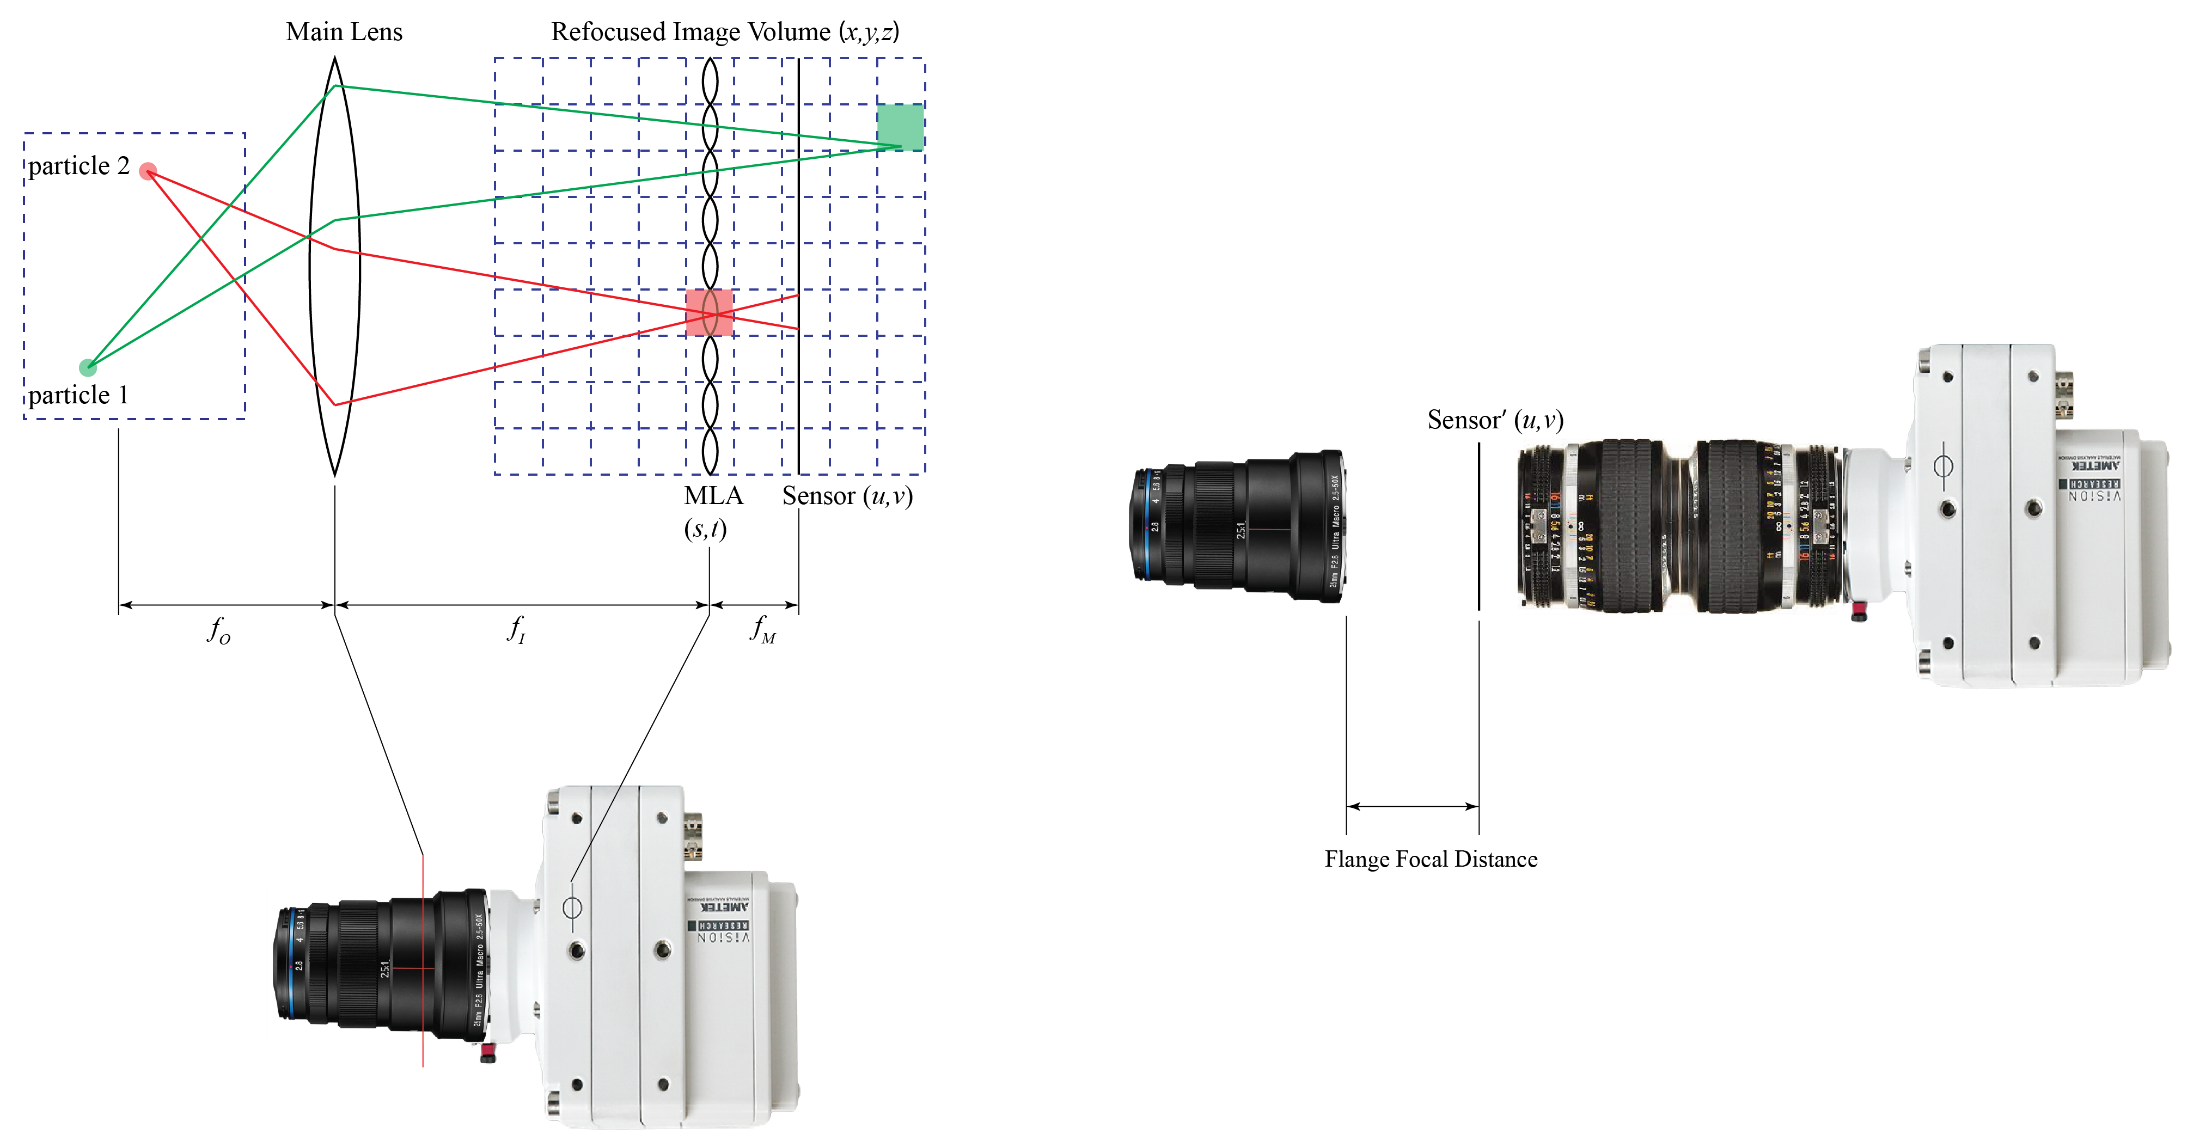
\includegraphics[width = 0.7\linewidth]{fig/ZoomLens_Setup.png}} 
  \caption{Light field system with 25mm $f$/2.8 2.5 $\times$ macro lens. 
  }
\label{fig:ZoomLens_Setup}
\end{figure}

\section*{1. Parallelized Ray Counting - pursue real-time tracking}
% I already finished this part actually,
% Just want to show partial result that I am working on that part. 
For cm-scale sparse particle tracking, providing near-instantaneous tracking result is essential function to apply this method to many applications such as controllable flow structure interactions, detection of micro-organism activities and so on. I decided to squeeze the power of modern processor to pursue real-time tracking. 
\autoref{fig:GPU} shows the raw LF images can be reorganized as 4 D matrix, each row will represent one pixel, which can be processed by single thread. Hence every pixel in each image will be processed simultaneously to reduce the reconstruction time. Consider the memory transfer latency, target volume is discretized into 400 $\times$ 200 $\times$ 150 voxels, 3D reconstruction time for single frame is compared for SIMD, OpenMP, MPI, CUDA method (\autoref{fig:running_time}). GPU-based parallel computing is as efficient as MPI method, but it can be executed in desktop instead of multi-nodes on super cluster.
\begin{figure}[h]
  \centerline{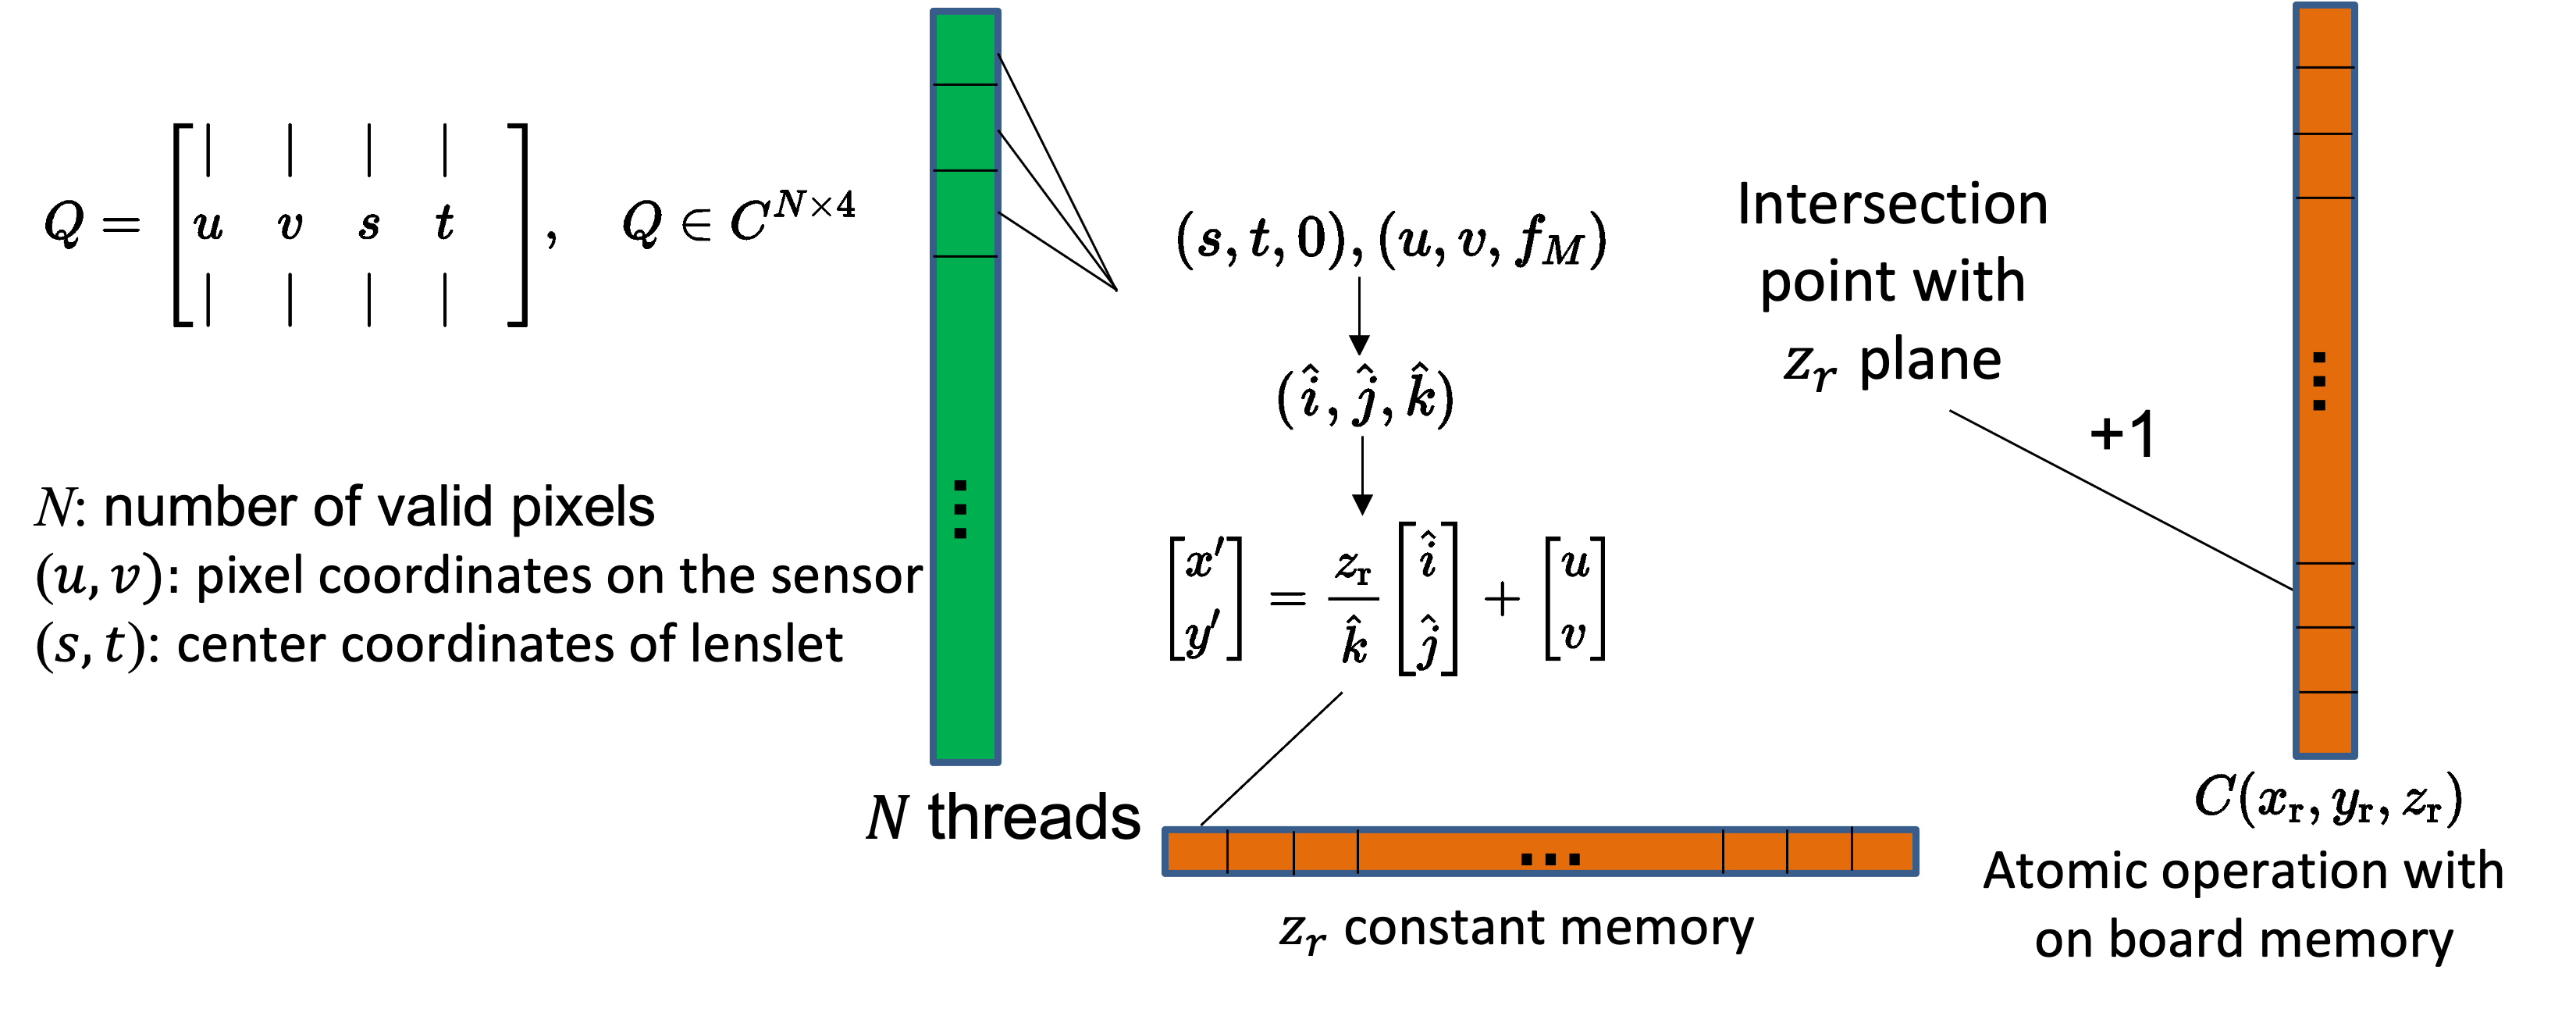
\includegraphics[width = 0.9\linewidth]{fig/GPU.png}} 
  \caption{Parallelized computing in GPU.}
\label{fig:GPU}
\end{figure}

\begin{figure}[h]
  \centerline{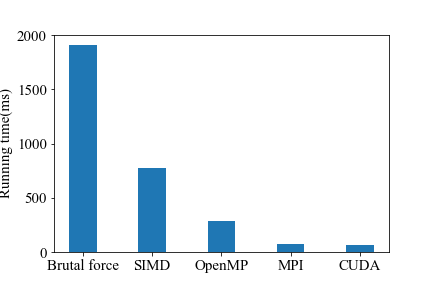
\includegraphics[width = 0.7\linewidth]{python/running_time.png}} 
  \caption{Computation time for SIMD, OpenMP, MPI, CUDA method.}
\label{fig:running_time}
\end{figure}
The future plan of this part is combine parallelized reconstruction step with updated classification step and tree searching step (\autoref{fig:flowchart})to achieve real-time tracking.

\section*{2. Lens Distortion - perspective view}
Compared to orthographic imaging system (microscopy), perspective zoom lens introduces larger lens distortion due to relative short effective focal length (EFL). \autoref{fig:compareOP} reveals that when approach to the edge of images, we can't use center of circle to represent the lenslet center in Zoom lens image due to significant distortion. For microscopical system, this distortion can be calibrated by reducing condense aperture size (\autoref{fig:distortion}). However, tuning aperture size of Zoom lens system will introduce pixel level displacement between elements in optical train, which will destroy the calibration. For this part, a image processing based calirbation will be developed to elimite distorted subimages and indentify lenslet center. 

\begin{figure}[h]
  \centerline{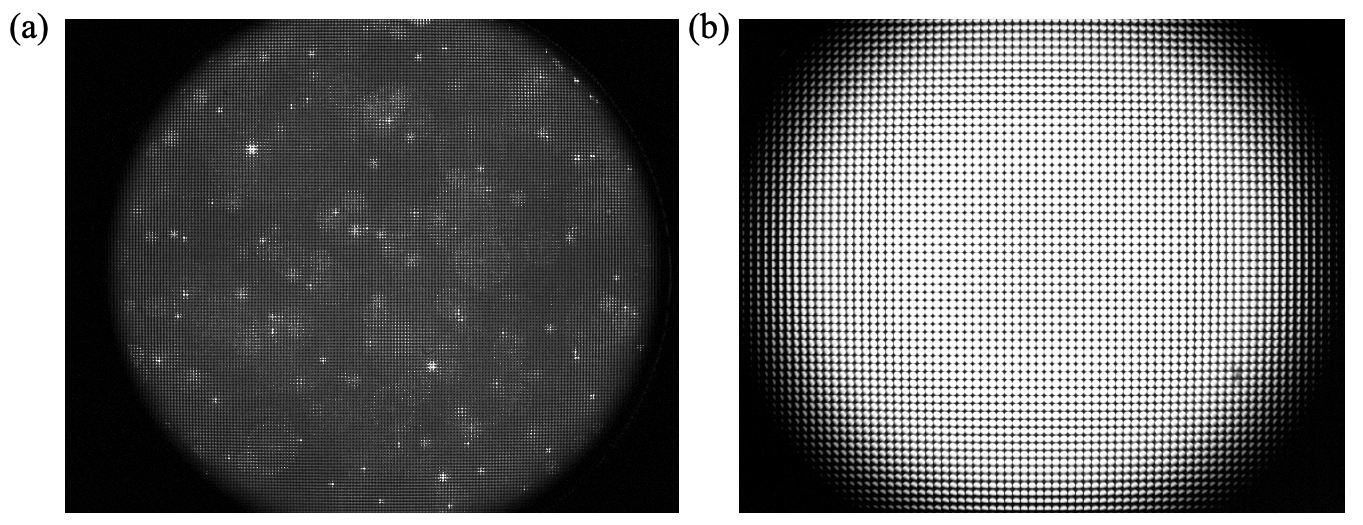
\includegraphics[width = 0.9\linewidth]{fig/CompareOP.png}} 
  \caption{(a) Orthographic calibration; (b) Zoom lens calibration. }
\label{fig:compareOP}
\end{figure}
\begin{figure*}[h]
  \centerline{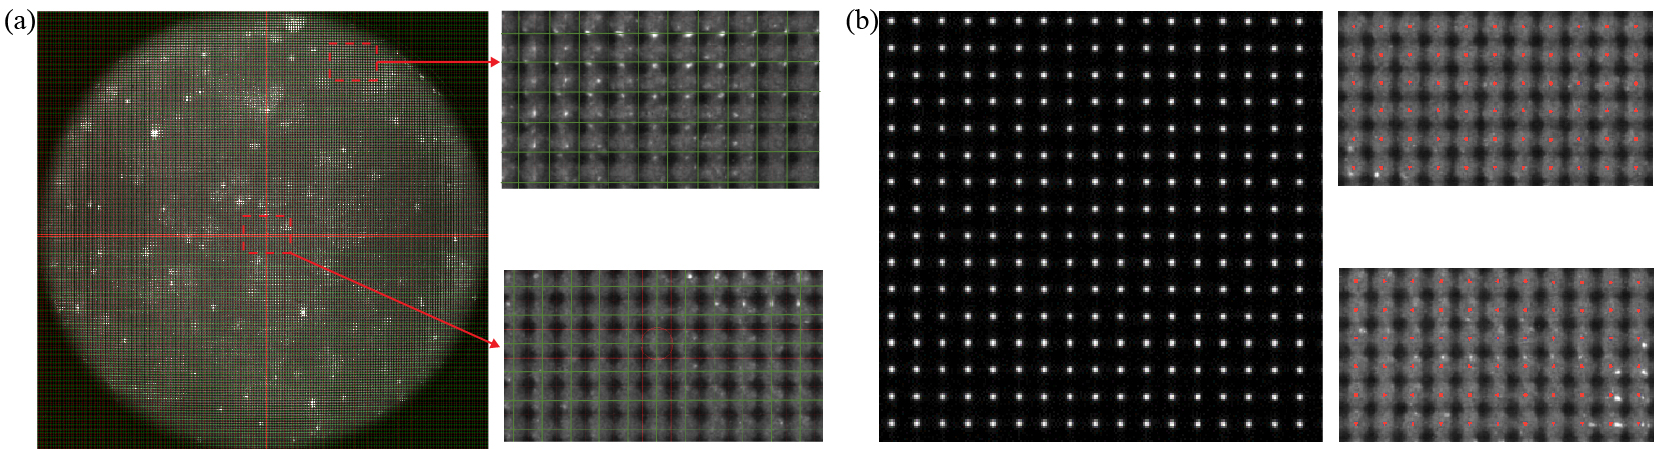
\includegraphics[width=1\linewidth]{fig/figure7.jpg}} 
  \caption{(a) An MLA grid overlaid on the image-based on the center alignment (grid points are center of each lenslet); (b) calibration images with small condenser aperture size, leading to precise micro image identification everywhere on the image (red points indicate the center of each lenslet).}
\label{fig:distortion}
\end{figure*}

\section*{3. Simulation}
In order to understand uncertainty in perspective view system, a physically-based simulation is inevitable. Based on $f/2.8$, 2.5 zoom-ratio Venus Laowa macro lens, which will be used in future experiment, we constructed a 12 elements $f/2.8$, 2.5 zoom-ratio macro lens (\autoref{fig:MLD}) \citep{smith2005modern} to perform particle reconstruction. With both 2D Zemax and 3D blender simulation, the uncertainty of short focal macro lens will be characterized. 

\begin{figure*}[h]
  \centerline{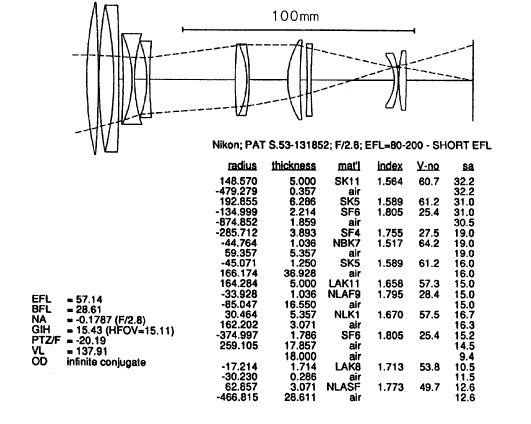
\includegraphics[width=0.7\linewidth]{fig/modern_lens_design.png}} 
  \caption{12-elements short focal macro lens.}
\label{fig:MLD}
\end{figure*}

\section*{4. Experiment}
We will use this approach to study the flow induced by oscillated boundary. Resonance speakers will be used to shake the boundary wall with various frequency and particle motion in 7mm $\times$ 7mm $\times$ 7mm volume will be captured by this LF camera system. 

\newpage
\bibliography{thesisbib}
%\bibliography{reference}
\bibliographystyle{plainnat}



\end{document}
\endinput
%%
%% End of file `thesis-ex.tex'.
